\chapter{Physical Implementation}

// TODO: add diagram of physical components and their connections

\section{Architecture}
The main specification the group had to meet at all costs was to be able to take a program (a sequence of instructions) as input, and output vector graphics on a screen.

Tracing the envisioned execution path of a program through the system gives insight into some of the considerations that had to be taken when designing the PCB and selecting components.

\begin{enumerate}
\item Assembled \vthreek programs are loaded into instruction memory via the EFM32 microcontroller.
\item The FPGA reads instructions from memory and performs execution.
\item The FPGA sends output via two interfaces, two DACs and an HDMI port.
\item The output from the DACs is displayed on an analogue oscilloscope and the output from the HDMI on a raster screen.
\end{enumerate}

\section{Components}
This section describes our choices of components.

The components had to meet our technical demands. Examples were number of pins, voltage level support, satisfying outputs, etc. We found this information, by inspecting the component datasheets.

The most important components are described in the next sections.

\subsection{MCU}
The MCU was an EFM32GG microcontroller from Silicon Labs. It served as an input processor for our system, handling input before and during run-time. Some of the technologies included with it, were also exploited, for instance buses.

\subsection{FPGA}
The FPGA was a Xilinx Spartan-6, with 401 kb block RAM. It served as the main processor in our design, fetching and executing instructions from instruction memory.

A JTAG header was connected to the FPGA for good accessibility to FPGA debugging and programming.
//TODO : elaborate

\subsection{SRAM}
Two SRAMs were put on our PCB. One of them worked as an instruction memory for the FPGA, while the other was a dedicated frame buffer for our output signals. The instructions executed in the FPGA would update the frame buffer, and data from the frame buffer could be read and transferred to the output units. 
Both SRAMs had an address space of 512k 16-bit words. 

\subsection{DACs and BNCs}
Since the purpose of our computer was to output vector graphics on an analogue vector screen, DACs were essential.
They would convert digital signals from the FPGA destined for the output screen, to corresponding analogue signals.

It was important that our DACs could output signals fast enough, to minimize flickering. Therefore, we chose DACs that could support clock rates up to 30MHz.

The BNCs connectors would receive the analogue signals and send them to the oscilloscope.
There was one DAC and one BNC for the x-coordinate and the same for the y-coordinate on the oscilloscope.

\subsection{Oscillators}
We connected two external oscillators to the MCU, one low frequency at 32,768kHz and one high frequency at 48MHz.
The MCU already contained internal RC-oscillators, but external oscillators were much more accurate and stable than the internal ones, which was important for avoiding more sources of errors.
Both crystals or full-fledged oscillators could be used, but our choice in the end was using oscillators.
The reason behind our choice, was that an oscillator was only one fully built component with all the necessary circuitry inside, and the datasheet clearly specified how it should be connected.
Crystals required load capacitors, whose values wasn't properly specified.
Another reason was that our FPGA explicitly needed an external oscillator, a crystal could not be used.
Hence, we chose oscillators for both the FPGA and MCU for simplicity.

The FPGA oscillator had a frequency of 100MHz.
Even though this was a high frequency, this signal could be scaled inside the FPGA to desirable frequencies.

\subsection{Buses}
Our system used one parallell bus (EBI) and one serial bus (SPI).
The MCU were bus master for both of them, since it supplied the bus technologies.

\subsubsection{EBI}
The FPGA, MCU and SRAM were connected via the EBI bus.
These connections were made properly by using the specified EBI-pins on the MCU. [citation to MCU datasheet]
The EBI bus allowed high-speed communication to the SRAM.
The EBI bus is a parallell bus, and we included the following bus lines in our implementation:
\begin{itemize}
\item 23 Address bits. It was more than we initially needed, but we couldn't be too sure.
\item 16 Data bits, since our SRAM consisted of 16-bit words.
\item 2 Chip select bits, one for the FPGA and one for the SRAM.
\item 1 Write enable bit, active low.
\item 1 Read enable bit, active low.
\end{itemize}

\subsubsection{SPI}
The SPI served as a three-way communication between the MCU, FPGA and Flash memory.
Its main purpose was to make our FPGA be configured from a bit-file stored in the flash memory.
As opposed to the EBI bus, SPI is a serial bus, transferring one bit of data at a time.

\subsection{Buttons and LEDS}
All buttons included a resistor for current limitation (to avoid short circuits) and pull-up (to avoid logical floating state).
The exception was the button connected to the MCU, where the pin had an internal pull-up.
All LEDs also included a current limiting resistor. 
Ohms law was used to calculate the required resistance [insert citation].

LEDs were handy for giving us an indication that something was turned on. For instance we had one LED which would light up, when the FPGA was configured.
Buttons were used for triggering events, like reset.

\subsection{Power Supply}
Our PCB would receive power from a micro-USB. A voltage level of 5V was sufficient, since we had no components which required more than 5V. However, we had plenty of components which required less than 5V, for instance 3.3V. To lower the voltage to a specific level, we used voltage regulators. Power is discussed in more detail in section \ref{Power}.

\subsection{Decoupling Capacitors}
Several major components required decoupling, e.g. the MCU, FPGA, voltage regulators, and DACs.
Decoupling means connecting power supplies through a capacitor network to ground, where power moving to ground can be temporarily stored.
This was necessary because it sometimes occurs situations where there is suddenly high need for power.
The power supply alone would not always be able to support these 'bursts'.
A capacitor network was the solution to this problem, as the component could pull power from the capacitors instead.

\section{PCB Design}
The architecture was realized on a printed circuit board (PCB) designed using Altium Designer 15.1.
Having never used this program before, the group had to overcome  challenges and difficulties related to not only learning new software, but also learning concepts of creating a PCB from scratch. 

\subsection{Schematics}
The entire logic of our PCB was designed with schematics. Altium allowed us to connect components together, pin by pin. Making the right connections was the only thing that mattered in the schematics. There was no focus on physical PCB-specific things like routing, component placement, etc.

When our schematics were completed, we moved on to design the physical PCB.

\subsection{Component Placement}
The goal was to place the components on the PCB, so that they preferably were in close range of all other components they had to connect with. 
This would shorten the routing, which was desirable in terms of mitigating signal delay and maintaining signal integrity.

The FPGA, SRAMs and MCU were the most important components with a lot of different connections, and were therefore placed central on the PCB.
I/O components, like controller buttons, USB, HDMI and BNC receptacles, were placed along the edge, since these were typically connected to few other components.
It would be annoying to connect external peripheral plugs to sockets in the middle of the PCB.

All decoupling capacitors involved in the decoupling network for a certain component, were placed in close proximity to that component.
This minimized the risk of that the component wouldn't get the extra power supply it needed during bursts.

All capacitors and resistors were placed on the bottom layer of the PCB to save space on an already crowded top layer.

\subsubsection{Component Footprints}
A component footprint is how the trace of a component looks like on the PCB.
In the beginning, component footprints from the standard Altium library were used.
After previewing the board, it became clear that these footprints were in fact gigantic, and footprints of suitable size had to be found using Altium vaults.
Smaller 0603 (1608 metric) footprints were used for most passive components, especially the capacitors and resistors.
By standardizing footprint sizes, the bill of materials could easily be updated without changing the PCB design, as long as the new component could be found in the same package size.
While a trade-off by using this small size package is that the components might be trickier to solder onto the board, the gain in size reduction for the board as a whole were valued higher by the group.
Some components could not be found in this footprint, but luckily there was no shortage of footprint sizes to choose from.

\subsection{Layers}
The PCB consisted of six signal layers: Top layer, bottom layer and four in between.
Two power layers were utilized: VCC and ground.

Between every signal and power layer a dielectric layer was added to make sure there was proper isolation between these conducting layers, so they wouldn't interfere with each other.

An overlay was added to both the top and bottom layers.
The overlay was added to contain silk-screen for marking components, thus making it easier to navigate the PCB.

The complete layer stack is shown in figure \ref{fig:Layers}

\begin{figure}[h!]
\centering
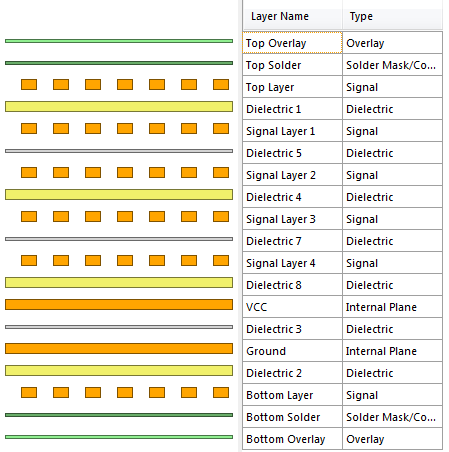
\includegraphics[scale = 0.8]{images/Layers.png}
\caption{Layer Stack}
\label{fig:Layers}
\end{figure}

\subsubsection{Power and ground}
\label{Power}
The PCB was designed with three power domains, each with their corresponding voltage regulator: 3.3V, 1.2V and a 5V reserved for analogue signals.
Most components were supplied by the 3.3V regulator, except for some internal parts of the FPGA that required 1.2V.

Since 3.3V was used by most components, and since only a few connectors required 1.2V, a dedicated power plane for 3.3V was added.
We also had a dedicated ground plane.
This saved us for yet more unnecessary routing, since everything connected to 3.3V or ground could go straight to a via by dogboning, and automatically be connected to the corresponding plane. The 1.2V traces were routed through all the connectors like any other signal. 

\subsubsection{Split planes}
The story of analogue 5V is a little different. The reason we had an analogue 5V, was to avoid noise from digital signals. The analogue components are sensitive to noise from the digital circuitry, and it was crucial for us to have as little noise as possible on the signal going to the oscilloscope. 
To avoid noise, the analogue and digital circuitry had to be separated completely. Analogue components could not use the same voltage supply as the digital ones and the same mattered for ground.
\newline
\newline
Our solution was to split the power and ground plane, shown in figure \ref{fig:Split planes}. 
\begin{itemize}
\item 5AV: Analogue 5V for components on the analogue plane. The reason it's 5V was because we weren't sure how much voltage the oscilloscope required to properly display the vector graphics from our program. 3.3V could be too low, so we went with 5V. Also, a high signal voltage could potentially help reduce noise.
\item AGND: Analogue components are connected to this ground instead of digital ground. This is to stop the analogue signal from getting disturbed by the digital signals on the ground plane.
\item 3.3V: Digital voltage for digital components.
\item GND: Digital ground.
\end{itemize}
All analogue components were placed in the analogue plane and the opposite with digital components. The exception was the DACs, which acts as a bridge between the digital part and the analogue part. These were placed on the actual split, with the affected pins on the correct side.
\newline
To remove any digital noise that could potentially accumulate on the analog ground plane, a diode was placed between the two ground planes, letting current flow from the analogue ground to the digital ground, but not vice versa.

\begin{figure}[h!]
\centering
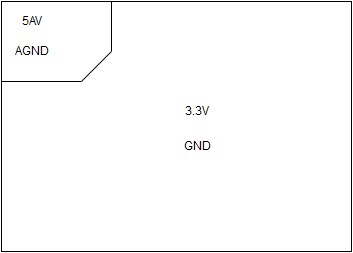
\includegraphics[scale = 0.6]{images/Split_planes.png}
\caption{Split between analogue and digital planes. The separating line is a solid, non-conducting material}
\label{fig:Split planes}
\end{figure}

\section{Routing}
The components had to be physically connected according to the schematics.
Connections could be manually routed or Altium's auto router could be used. The auto router would automatically route as many connections as possible.  

Routing was a much more time-consuming process than we expected. We had put too much trust into the built-in auto router in Altium. The router did not, as we naively thought, magically solve the routing. 
\subsection{Design Rules}
Before routing, necessary rules had to be defined to make sure the PCB was routed properly. The following listing explains the most important rules for our design.
\begin{itemize}
\item Clearance: 0.1mm. 
\newline
Minimum clearance between different traces
\item Width: 0.127mm, Power Width 0.203mm.
\newline
Minimum width for traces. Power traces had bigger minimum widths, than signal traces.
\item Via Diameter: 0.4mm, Via Hole Size: 0.2mm
\newline
Minimum diameter and hole size for multi-layer vias.
\item Short-circuits and net antennas not allowed
\end{itemize}
The rules were set like this to make sure there wouldn't be any interference between traces, while the traces were still wide enough to not be damaged by the signal itself. Power traces were wider to make sure they could handle the voltage. 
\newline
Net antennas were traces that lead to dead-ends. This could harm the design, since these dead-ends could work as unwanted signal receivers from nearby sources.
\newline
\subsubsection{Design Rule Check}
Altium had its own tool for testing how many violations our current design created, called Design Rule Check. It displayed the amount of errors occurred from each type, and the coordinates on the PCB for every error. 
Typical errors during our design procedure were short-circuits, net antennas and clearance constraint violations.
\subsection{Routing Procedure}
The task of routing the PCB was started by routing some components manually. We quickly discovered that doing this for the entire board would take a very long time, and so began to check out Altium's built-in auto router. 
\newline
\newline
Roughly, we followed this routing procedure:
\begin{enumerate}
\item Run the auto router.
\item Run Design Rule Check, and see how many errors that occured. 
\item If there are too many errors (e.g. more than 200), there is most likely something wrong with the design rules or the auto router settings. If not, go to step 6.
\item Check and modify settings and rules.
\item Go back to step 1.
\item Go through the remaining errors and fix them. 
\item ...
\item PROFIT!
\end{enumerate}
We ran into many different routing problems, which is discussed in detail in section \ref{Routing Problems}

\section{Fault Handling}
The team were all inexperienced with PCB design and often uncertain if actions or decisions could cause problems down the line. The top priority was to make something that worked properly. A failing component was not unusual, and forgetting something was almost guaranteed to happen, considering the vast amount of factors involved. Hence, having back-up features was critical to us.
\subsection{Headers}
Our primary strategy of redundancy was including headers. A lot of headers. Our final amount of headers ended up at 34, including the JTAG and the ARM programming header. This would make us able to measure most signals with a multimeter and verify them. 
\newline
Pretty much every header was between components. If wrong connections existed, or a connection didn't work, we could use headers to easily correct the connections, by soldering on wires. Not only could we detect errors, but also fix them.

\begin{figure}[h!]
\centering
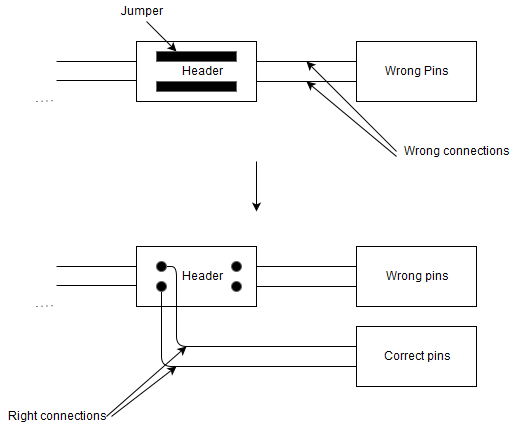
\includegraphics[scale = 0.45]{images/Header_fix.png}
\caption{Example Header fix}
\label{fig:Header fix}
\end{figure}

Headers was also useful as switches. By manually connecting header pins with jumpers, we could activate and deactivate certain parts of the PCB. This would be useful when focusing on lesser parts of the circuit. For instance, we used 3-pin headers to give us the ability of manually turning on and off different voltage levels. 

We could also deliver power to the components directly through the headers, if any issue with the power supply would occur.

\subsection{DACs}
Even though we had our own DACs for outputting analog voltage out to the BNC plug, there was still a risk that we could not get them to work at all. We had a back-up solution by also connecting the internal DACs in the MCU to the BNCs. One 2x2 header for each BNC input was used, to manually control if we wanted to use the main DACs or the MCU DACs. This is described in figure \ref{fig:DAC headers}. There's one header each for the X and the Y signal to the oscilloscope. 

\begin{figure}[h!]
\centering
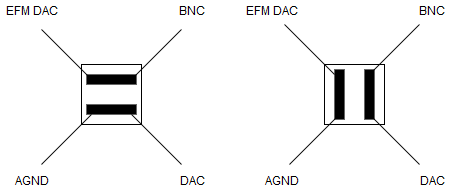
\includegraphics[scale = 0.6]{images/DAC_headers.png}
\caption{Left: Jumpers connecting MCU DAC to BNC and normal DAC to ground.
         Right: The opposite}
\label{fig:DAC headers}
\end{figure}

